\documentclass[10pt,xcolor=table ]{beamer}
	
\usetheme{metropolis}
\usepackage{appendixnumberbeamer}

\usepackage{booktabs}
\usepackage[scale=2]{ccicons}

\usepackage{pgfplots}
\usepgfplotslibrary{dateplot}

\usepackage{xspace}
\usepackage{graphicx}
\usepackage{graphics}


\usepackage[spanish]{babel}
\usepackage[utf8]{inputenc}

\usepackage{decorule}
\newcommand{\decoRule}{\rule{\textwidth}{.4pt}} % New command for a rule to be used under figures


\usepackage{pgf-pie}
\usepackage{pgfplots}

\usepackage[export]{adjustbox}


\definecolor{UniBlue}{RGB}{255,255,255}
\setbeamercolor{background canvas}{bg=UniBlue}


\title{Desarrollo de un sistema de gestión de programas de estudio orientado a resultados pedagógicos}
\subtitle{Proyecto final de la carrera}
\author{Luis Fernando Villalba Vera}
\institute{Universidad Católica - Nuestra Señora de la Asunción}
\date{\today}
\titlegraphic{\hfill
\includegraphics[height=1.5cm]{../Figuras/uca}}

\begin{document}

\maketitle

\begin{frame}{Contenido}
	\begin{enumerate}
	    \item Justificación
	    \item Objetivos
	    \item Estado del arte
	    \item Marco teórico
	    \item Caso de estudio
	    \item Propuesta de trabajo
	    \item Proceso de desarrollo
	    \item Validación del desarrollo
	    \item Conclusión y aportes
	 \end{enumerate}
\end{frame}

% JUSTIFICACIÓN
\section{Justificación}
\begin{frame}{Conceptos}
  \begin{itemize}[<+- | alert@+>]
    \item Problemática
    \item Competencias académicas y su evaluación
    \item Sistemas de gestión de evaluaciones (AMS)
    \item Sistemas de gestión curricular (CMS)
  \end{itemize}
\end{frame}

\subsection{Diseño de cursos y programas}
\begin{frame}{Diseño de cursos y programas}
	\begin{figure}
		\centering
	    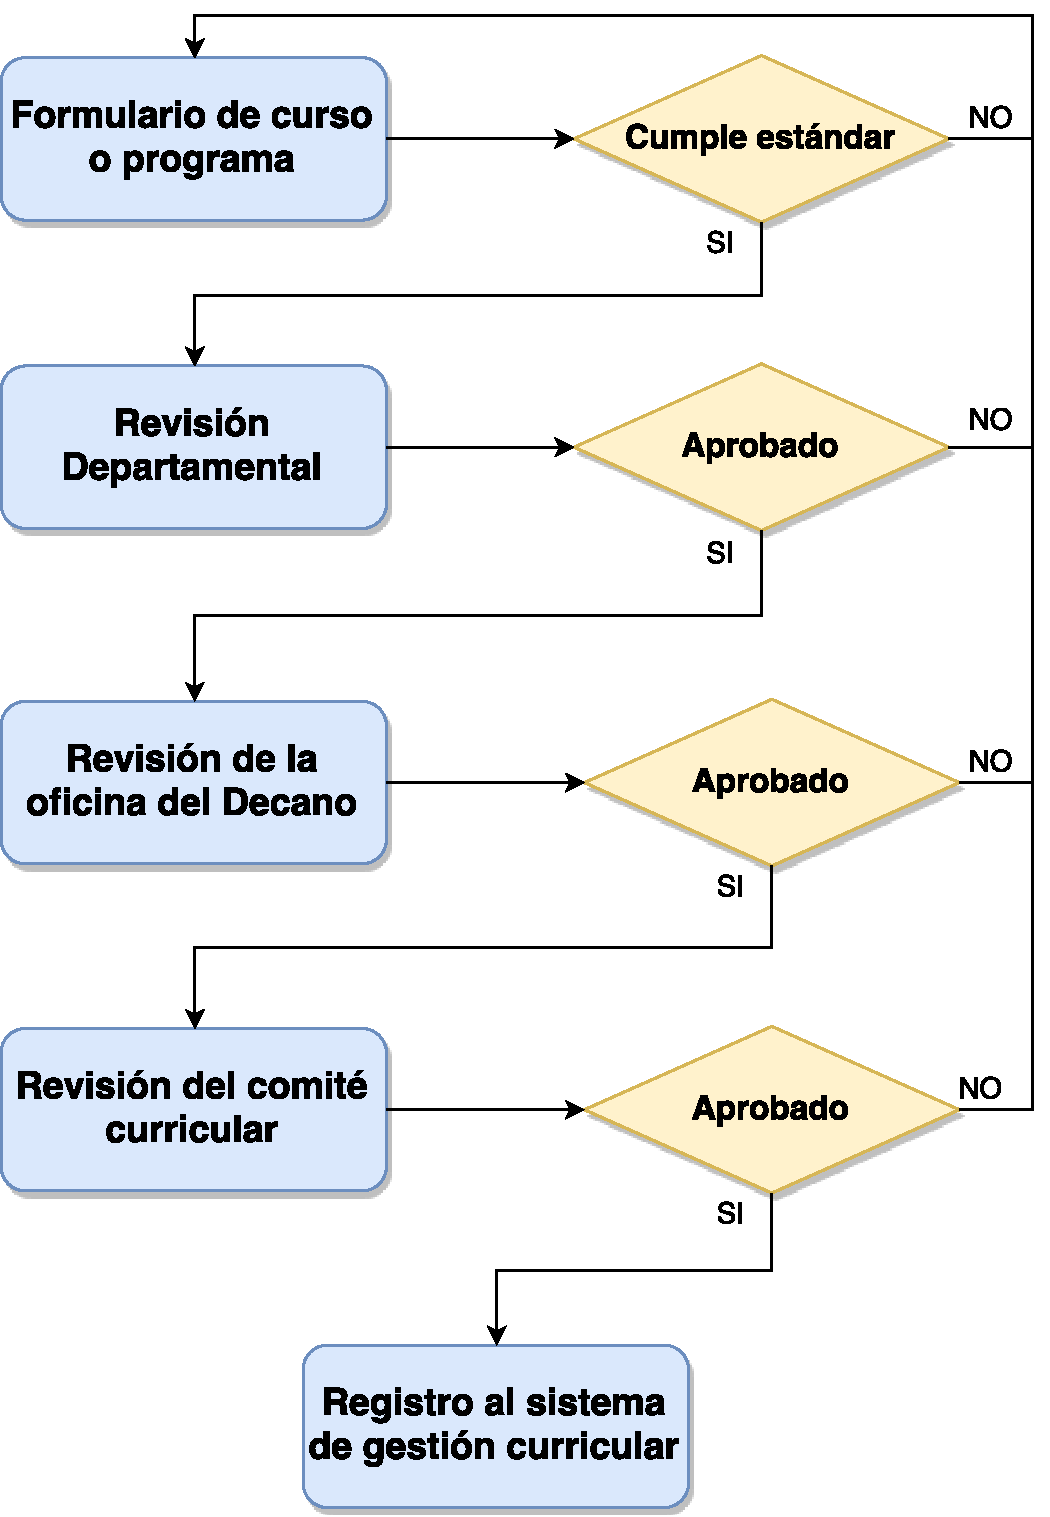
\includegraphics[scale=0.3]{../Figuras/course_creation_flow}
	\end{figure}
\end{frame}

\subsection{Disponibilidad en el sistema de gestión de competencias}
\begin{frame}{Disponibilidad en el sistema de gestión de competencias}
	\begin{figure}
		\centering
	    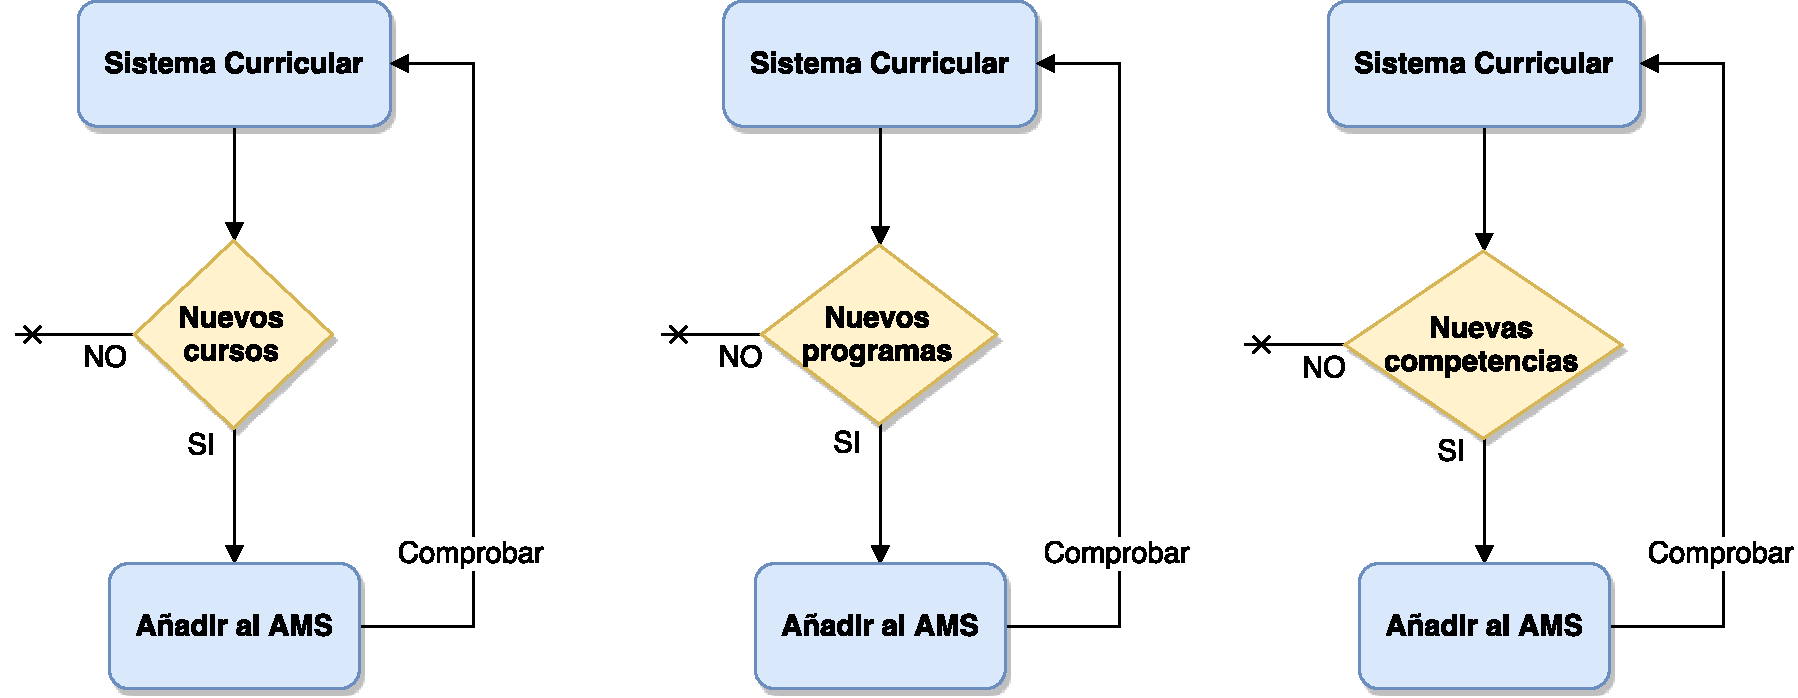
\includegraphics[scale=0.35]{../Figuras/after_creation}
	\end{figure}
\end{frame}

% OBJETIVOS
\section{Objetivos}
\subsection{Objetivos}
\begin{frame}[t]{Objetivos}
	\metroset{block=fill}
	\begin{alertblock}{Objetivo general}
        Diseñar una aplicación que permita integrar y estructurar tareas separadas de un sistema académico para una gestión de programas educativos orientados a resultados pedagógicos, que provea soporte a flujos de trabajo para sus diferentes etapas de aprobación.
      \end{alertblock}

	\metroset{block=fill}
	\begin{alertblock}{Objetivos específicos}
        \begin{itemize}
        	\item Realizar un relevamiento de los requerimientos, diseño e implementación de un sistema de gestión de programas orientado a competencias.
        	\item Realizar el proyecto en un marco de programación ágil, estimando y desarrollando la aplicación de acuerdo a las directrices brindadas por la metodología.
        	\item Validar la herramienta desarrollada: con expertos del dominio principalmente y de manera preliminar con experiencias limitadas con los usuarios finales.
        \end{itemize}
    \end{alertblock}
\end{frame}

% ESTADO DEL ARTE
\section{Estado del arte}
\subsection{Sistemas de gestión curricular}
\begin{frame}{Sistemas de gestión curricular}
	\begin{figure}
		\centering
	    
\includegraphics[scale=0.5]{../Figuras/cms_alternatives}
	\end{figure}
\end{frame}

\subsection{Comparación de sistemas relacionados}
\begin{frame}{Comparación de sistemas relacionados}
  	\begin{table}[H]
  	\small
	\centering
	\resizebox{\columnwidth}{!}{%
		\begin{tabular}{lllccl}
		\toprule
		\multicolumn{3}{l}{Características}                                                & CurricUNET                       & CourseLeaf            & DECA         \\
		\midrule
		\rowcolor[HTML]{ECF4FF}
		\multicolumn{3}{l}{Creación y versionamiento de competencias.}                     &                                  &                       &              \\
		\multicolumn{3}{l}{Creación y versionamiento de cursos.}                           & $\checkmark$                     & $\checkmark$          & $\checkmark$ \\
		\multicolumn{3}{l}{Creación y versionamiento de programas de estudio.}             & $\checkmark$                     & $\checkmark$          &              \\
		\multicolumn{3}{l}{Cumple los Estándares de códigos de California.} 			   & $\checkmark$                     &                       &              \\
		\rowcolor[HTML]{ECF4FF}
		\multicolumn{3}{l}{Historial de versiones de competencias.}     			       & 			                      & 		              &  			 \\
		\multicolumn{3}{l}{Historial de versiones de cursos.}     			               & $\checkmark$                     & $\checkmark$          & $\checkmark$ \\
		\multicolumn{3}{l}{Historial de versiones de programas de estudio.}     		   & $\checkmark$                     &  			          & 			 \\
		\multicolumn{3}{l}{Reporte de Comparación entre versiones de cursos.}              & 			                      &                       & $\checkmark$ \\
		\rowcolor[HTML]{ECF4FF}
		\multicolumn{3}{l}{Soporta competencias de aprendizaje del estudiante.}            &                      			  &                       &              \\
		\multicolumn{3}{l}{Plantilla de flujo de trabajo customizable.}                    & $\checkmark$                     &                       &              \\
		\multicolumn{3}{l}{Permite asignar roles evaluadores en la aplicación.}            & $\checkmark$                     & $\checkmark$          &              \\
		\multicolumn{3}{l}{Permite asignar usuarios como colaboradores.}                   & $\checkmark$                     &                       &              \\
		\multicolumn{3}{l}{Soporte de correlatividades entre cursos.}                      & $\checkmark$ 					  &						  &              \\
		\multicolumn{3}{l}{Incluye un catálogo de cursos.}                   		   	   & $\checkmark$					  &	$\checkmark$		  & $\checkmark$ \\
		\multicolumn{3}{l}{Incluye un catálogo de programas de estudio.}                   & $\checkmark$					  &	            		  &              \\
		\rowcolor[HTML]{ECF4FF}
		\multicolumn{3}{l}{Incluye un catálogo de competencias.}                   	       & 								  &						  & 			 \\
		\multicolumn{3}{l}{UX intuitiva y efectiva.}     			   					   &                                  & $\checkmark$          & $\checkmark$ \\
		\bottomrule
		\end{tabular}
	}
	\end{table}
\end{frame}

% MARCO TEORICO
\section{Marco teórico}
\subsection{Software as a Service}
\begin{frame}{Software as a Service}
	\metroset{block=fill}
	\begin{alertblock}{Definición}
		Paradigma de entrega de software como servicio a través de una red.
	\end{alertblock}

	\begin{columns}[c,onlytextwidth]
    	\column{0.6\textwidth}
		\begin{block}{Características}
			\begin{itemize}
	        	\item Modelo de suscripción.
	        	\item Acceso y administración a través de una red.
	        	\item Actividades gestionadas desde ubicaciones centrales.
	        	\item Actualizaciones centralizadas.
	      		\item Arquitectura multi-tenant.
	    	\end{itemize}
		\end{block}
	    \column{0.4\textwidth}
		\begin{figure}[H]
			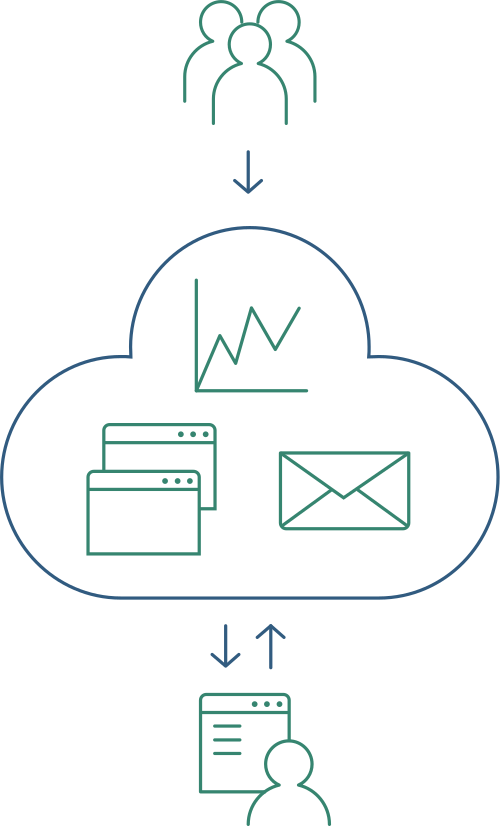
\includegraphics[scale=0.23]{../Figuras/saas}
		\end{figure}
  	\end{columns}
\end{frame}

\subsection{Sistemas de gestión de evaluaciones}
\begin{frame}{Sistemas de gestión de evaluaciones}
	\begin{figure}
		\centering
	    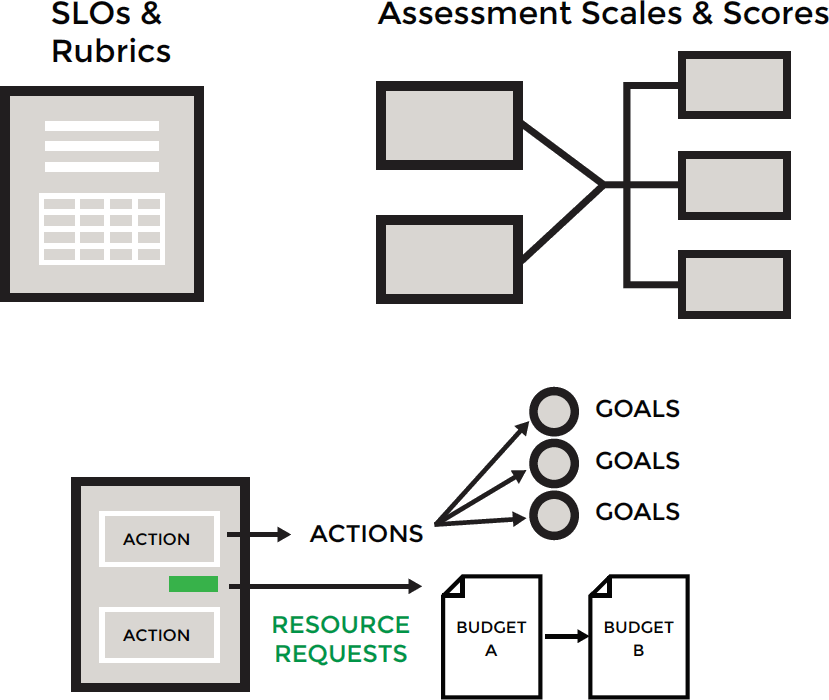
\includegraphics[scale=0.55]{../Figuras/ams}
	\end{figure}
\end{frame}

\subsection{Metodología ágil}
\begin{frame}{Metodología ágil}
	\metroset{block=fill}
	\begin{alertblock}{Definición}
		Enfoque para toma de decisiones basado en el desarrollo iterativo e incremental.
	\end{alertblock}

	\begin{columns}[c,onlytextwidth]
    	\column{0.5\textwidth}
		\begin{block}{Características}
			\begin{itemize}
	        	\item Entregas de valor agregado en iteraciones.
	        	\item Adaptación al cambio.
	        	\item El cliente es parte del proceso de desarrollo.
	    	\end{itemize}
		\end{block}
	    \column{0.5\textwidth}
		\begin{figure}
		    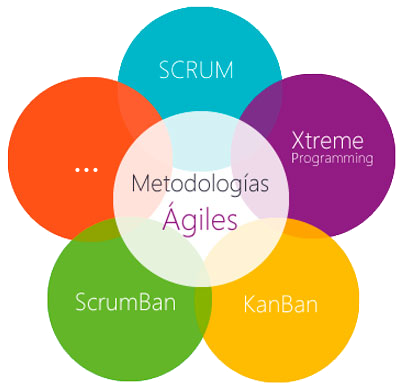
\includegraphics[scale=0.32]{../Figuras/met_agiles}
		\end{figure}
  	\end{columns}
\end{frame}

\subsection{Interacción Humano-Computador}
\begin{frame}{Interacción Humano-Computador}
	% \metroset{block=fill}
	% \begin{alertblock}{Definición}
	% 	Enfoque para toma de decisiones basado en el desarrollo iterativo e incremental.
	% \end{alertblock}

	% \begin{columns}[c,onlytextwidth]
 %    	\column{0.5\textwidth}
	% 	\begin{block}{Características}
	% 		\begin{itemize}
	%         	\item Entregas de valor agregado en iteraciones.
	%         	\item Adaptación al cambio.
	%         	\item El cliente es parte del proceso de desarrollo.
	%     	\end{itemize}
	% 	\end{block}
	%     \column{0.5\textwidth}
	% 	\begin{figure}
	% 	    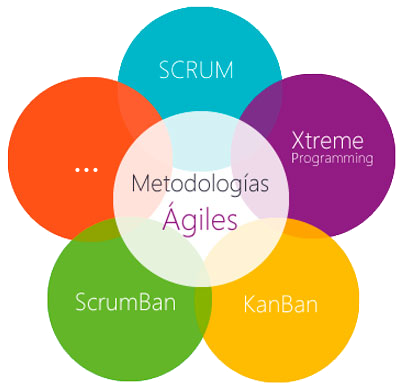
\includegraphics[scale=0.32]{../Figuras/met_agiles}
	% 	\end{figure}
 %  	\end{columns}
\end{frame}

% CASO DE ESTUDIO
\section{Caso de estudio}
\subsection{Caso de estudio}
\begin{frame}{Caso de estudio}
  	Caso de estudio de observación participante: desarrollo de un sistema de curriculums orientado a competencias.

	\begin{block}{Requerimientos no funcionales}
		\begin{itemize}
			\item Arquitectura Software as a Service.
			\item Utilización de abordaje ágil de desarrollo.
    	\end{itemize}
	\end{block}
\end{frame}

% PROPUESTA DE TRABAJO
\section{Propuesta de trabajo}
\subsection{Módulo de gestión curricular integrado a un AMS}
\begin{frame}{Módulo de gestión curricular integrado a un AMS}
	\begin{figure}
		\centering
	    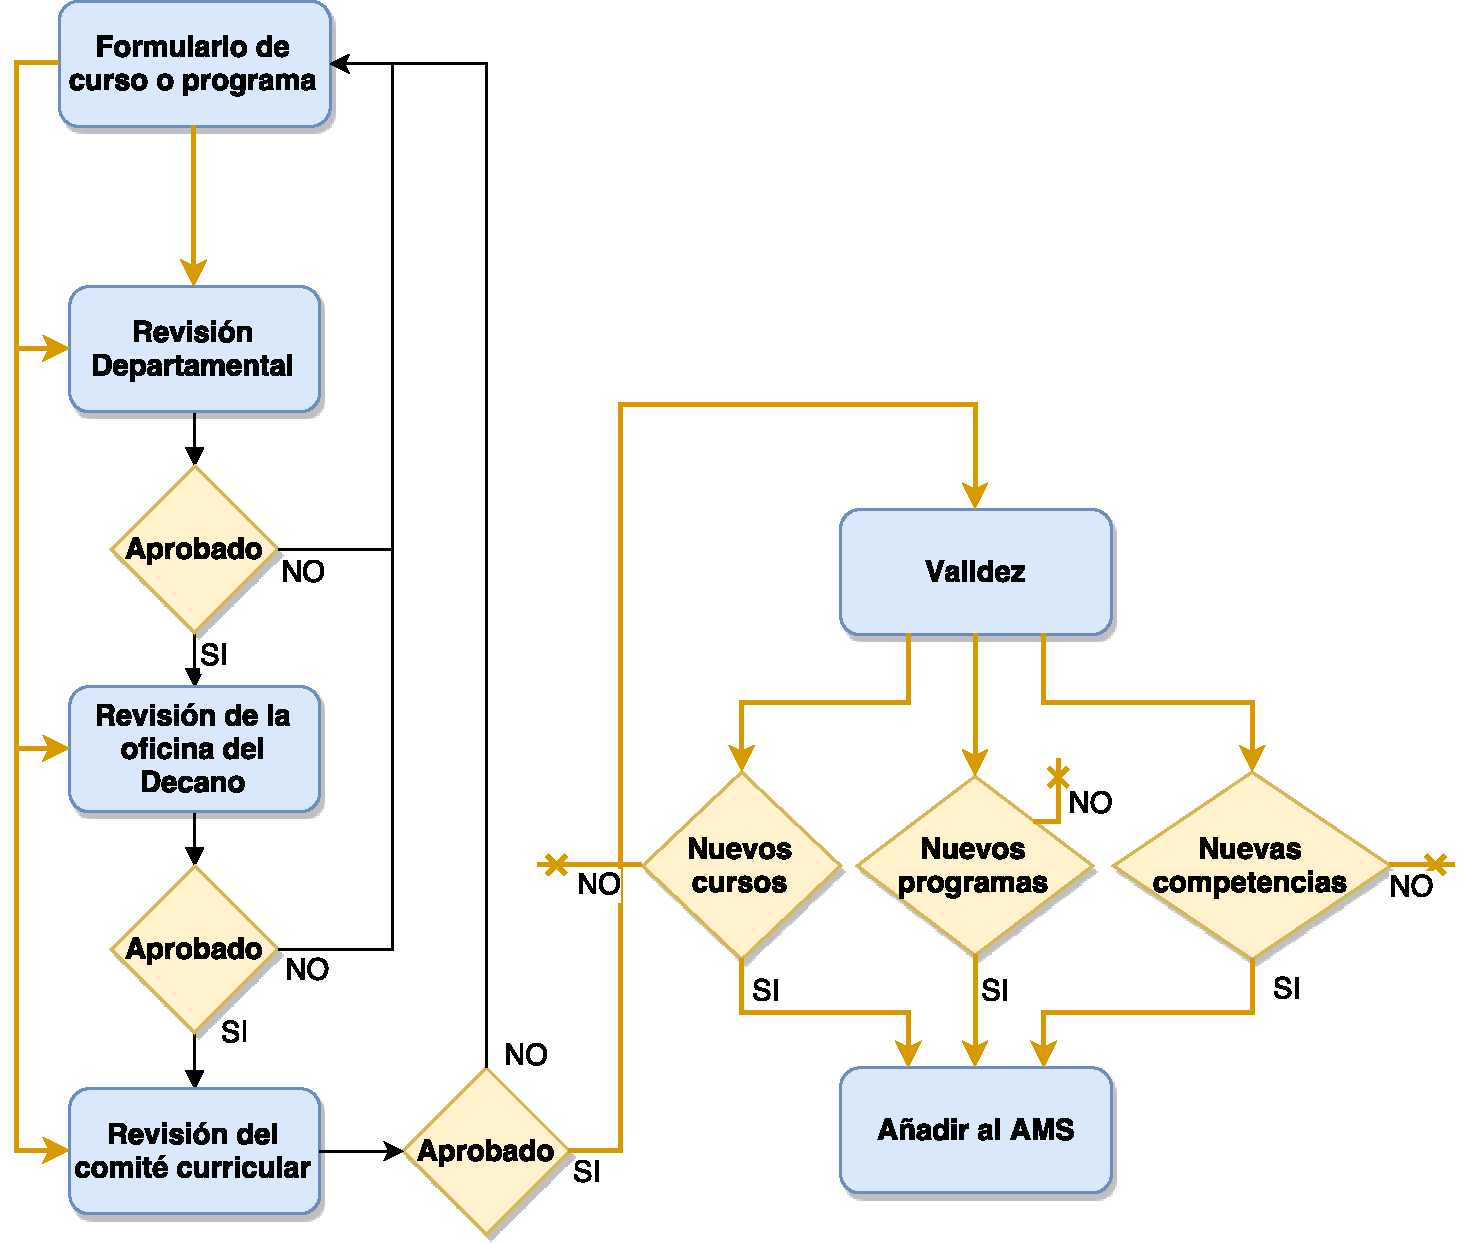
\includegraphics[scale=0.25,left]{../Figuras/proposal}
	\end{figure}
\end{frame}

\begin{frame}{Modelo de la propuesta de solución}
	\begin{figure}
		\centering
	    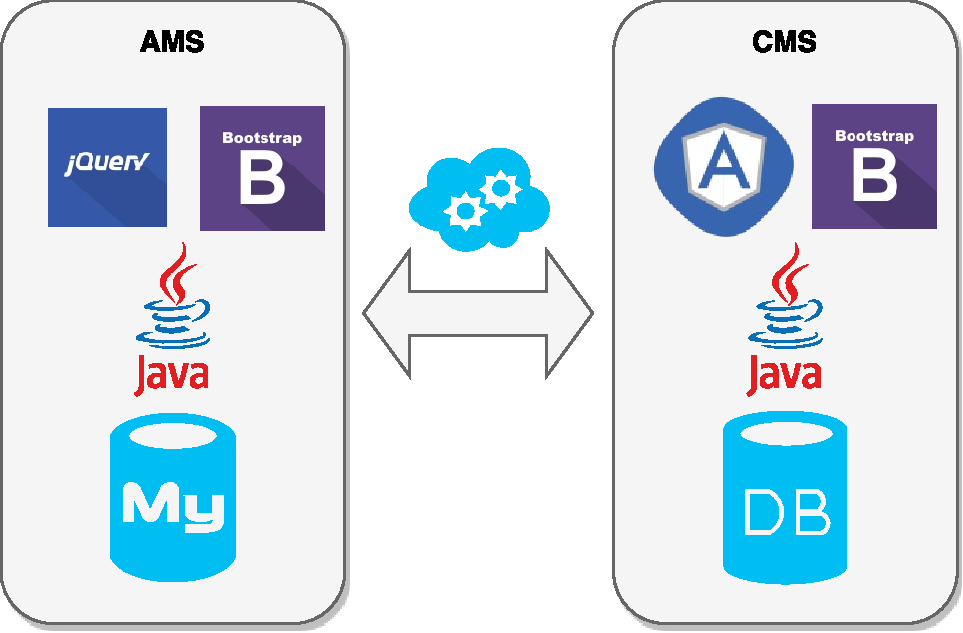
\includegraphics[scale=0.55]{../Figuras/architecture}
	\end{figure}
\end{frame}

% PROCESO DE DESARROLLO
\section{Proceso de desarrollo}
\subsection{Definición de épicas e historias de usuario}
\begin{frame}{Definición de épicas e historias de usuario}
	\begin{figure}
		\centering
	    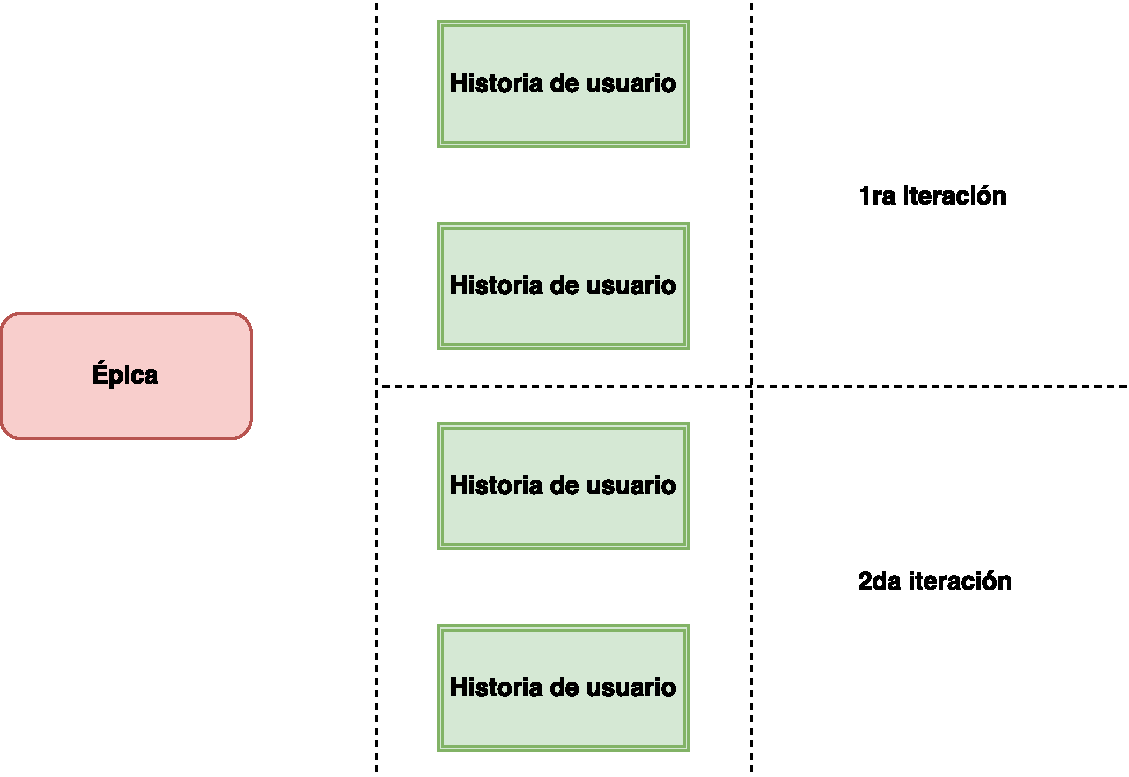
\includegraphics[scale=0.5]{../Figuras/epic_diagram}
	\end{figure}
\end{frame}

\subsection{Flujo del desarrollo}
\begin{frame}{Flujo del desarrollo}
	\begin{figure}
		\centering
	    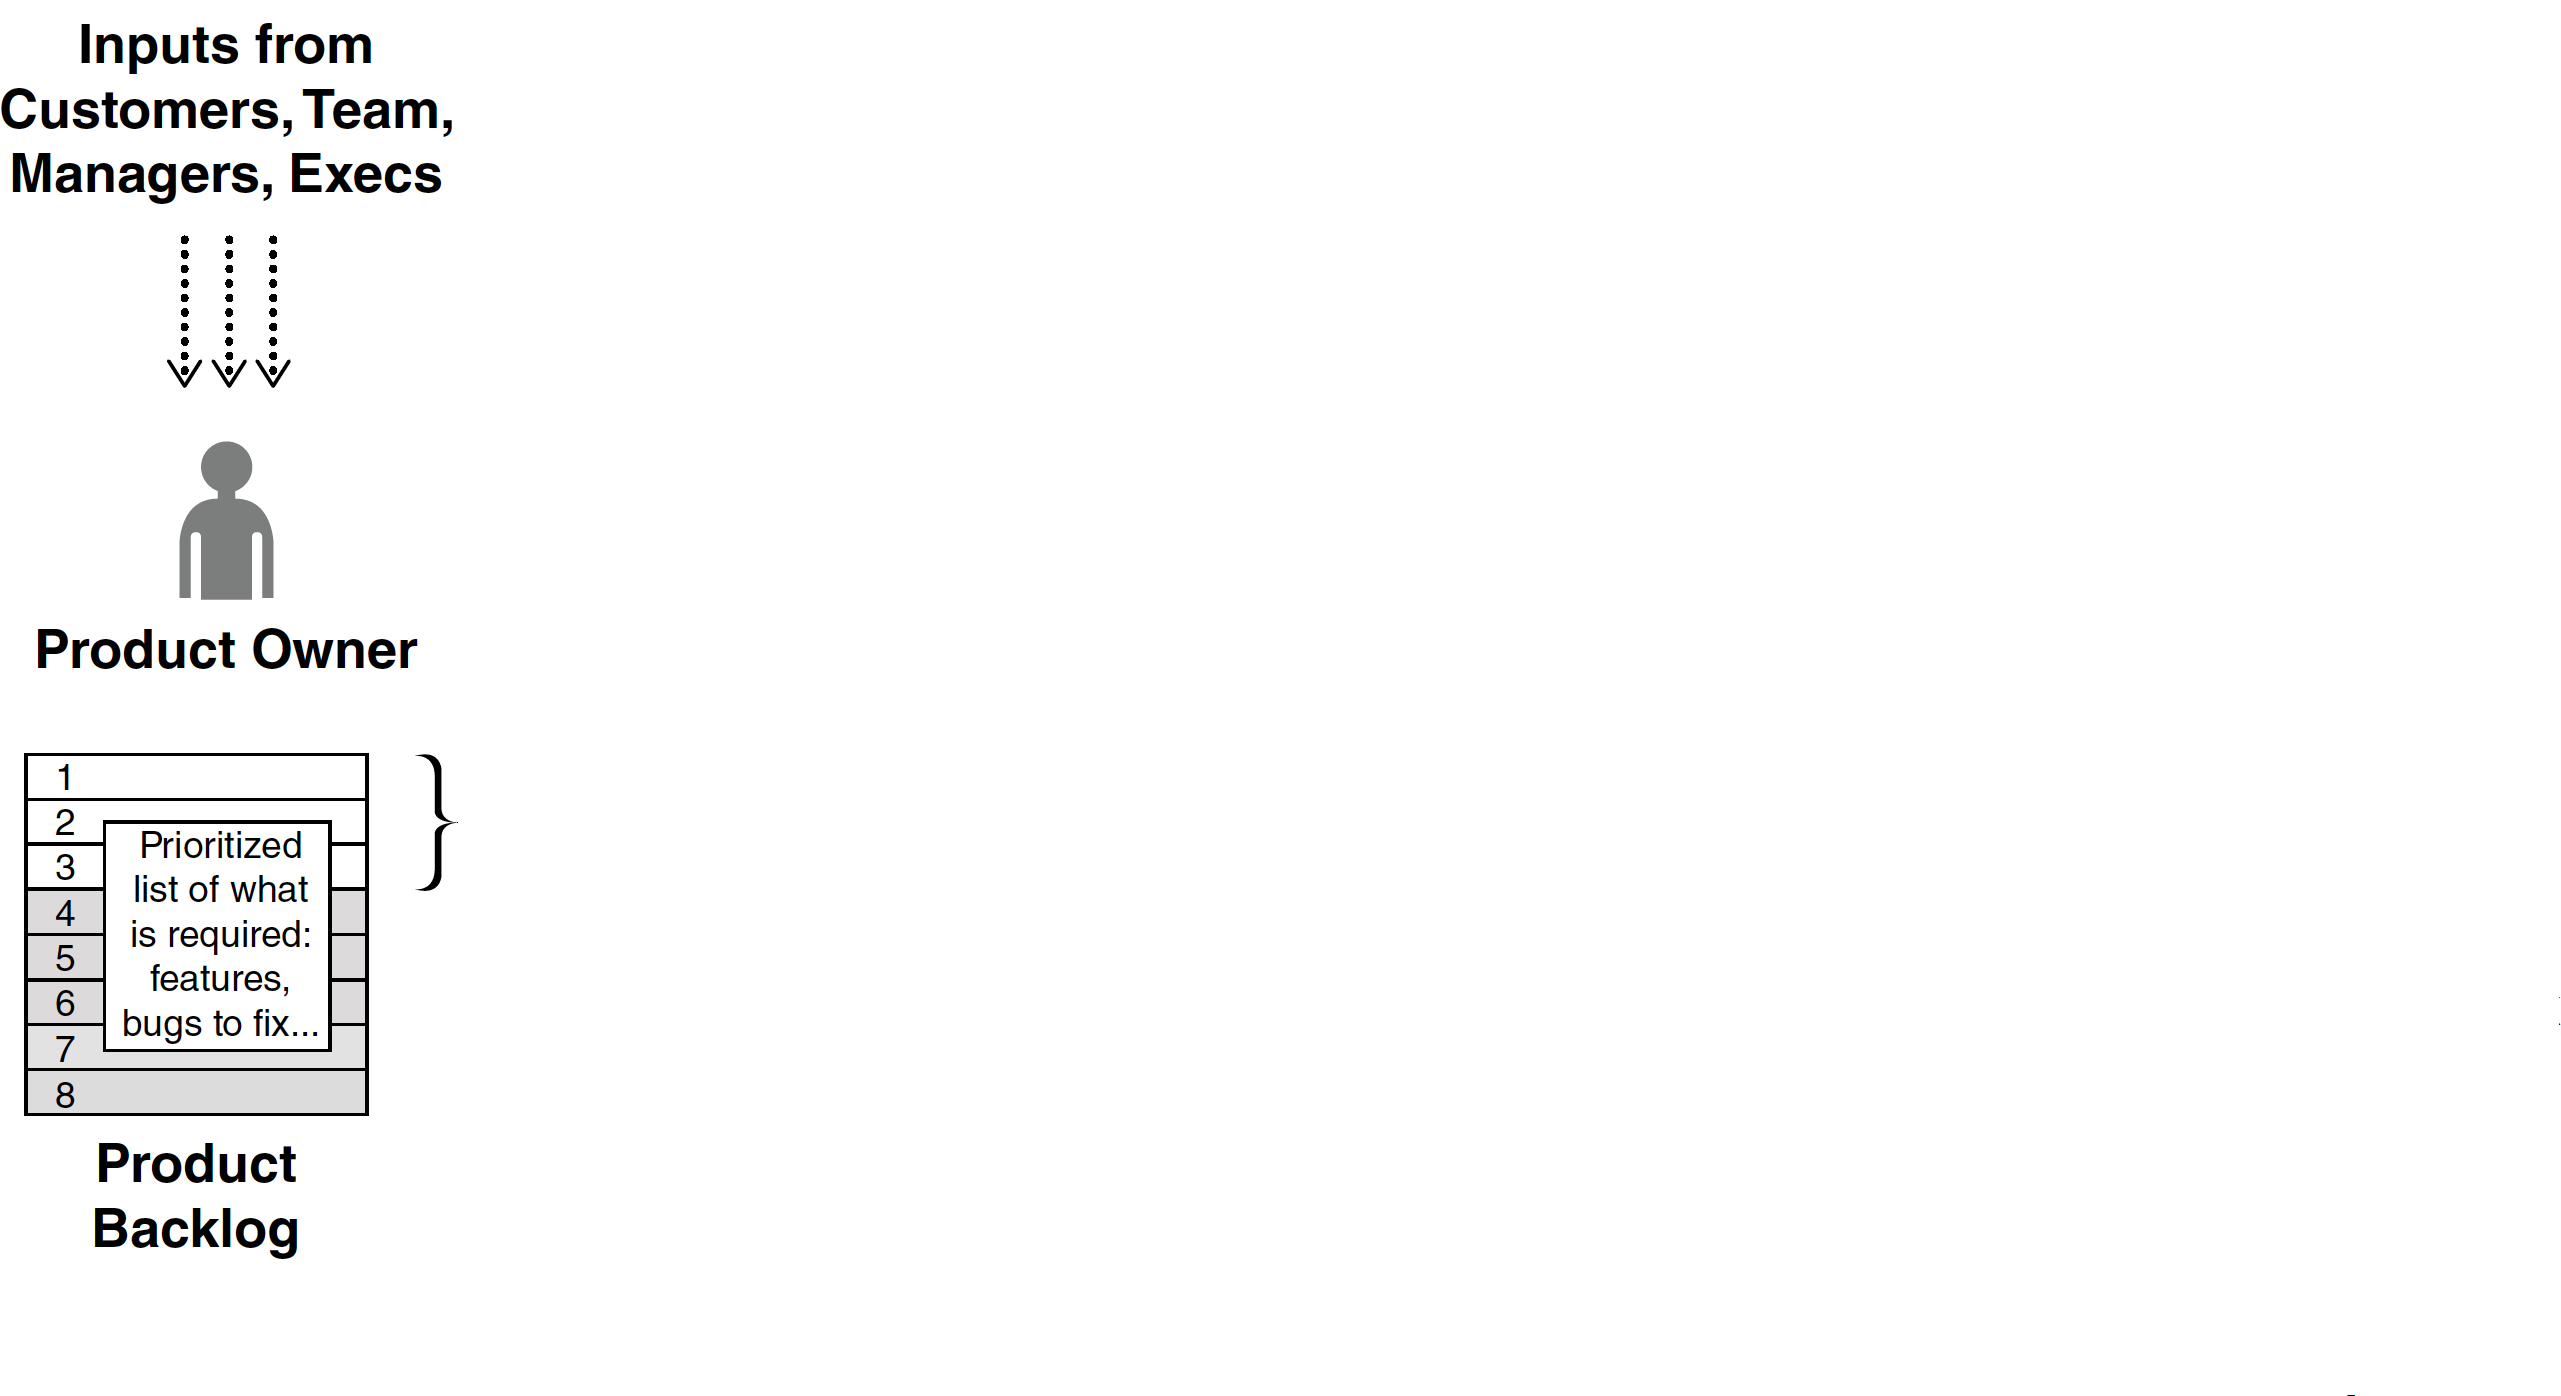
\includegraphics[scale=0.235]{../Figuras/flujo_scrum_1}
	\end{figure}
	\decoRule \\
  	\tiny \textit{Charles G Cobb. The project manager’s guide to mastering Agile: Principles and practices for an adaptive approach. John Wiley \& Sons, 2015.} \\
\end{frame}

\begin{frame}{Flujo del desarrollo}
	\begin{figure}
		\centering
	    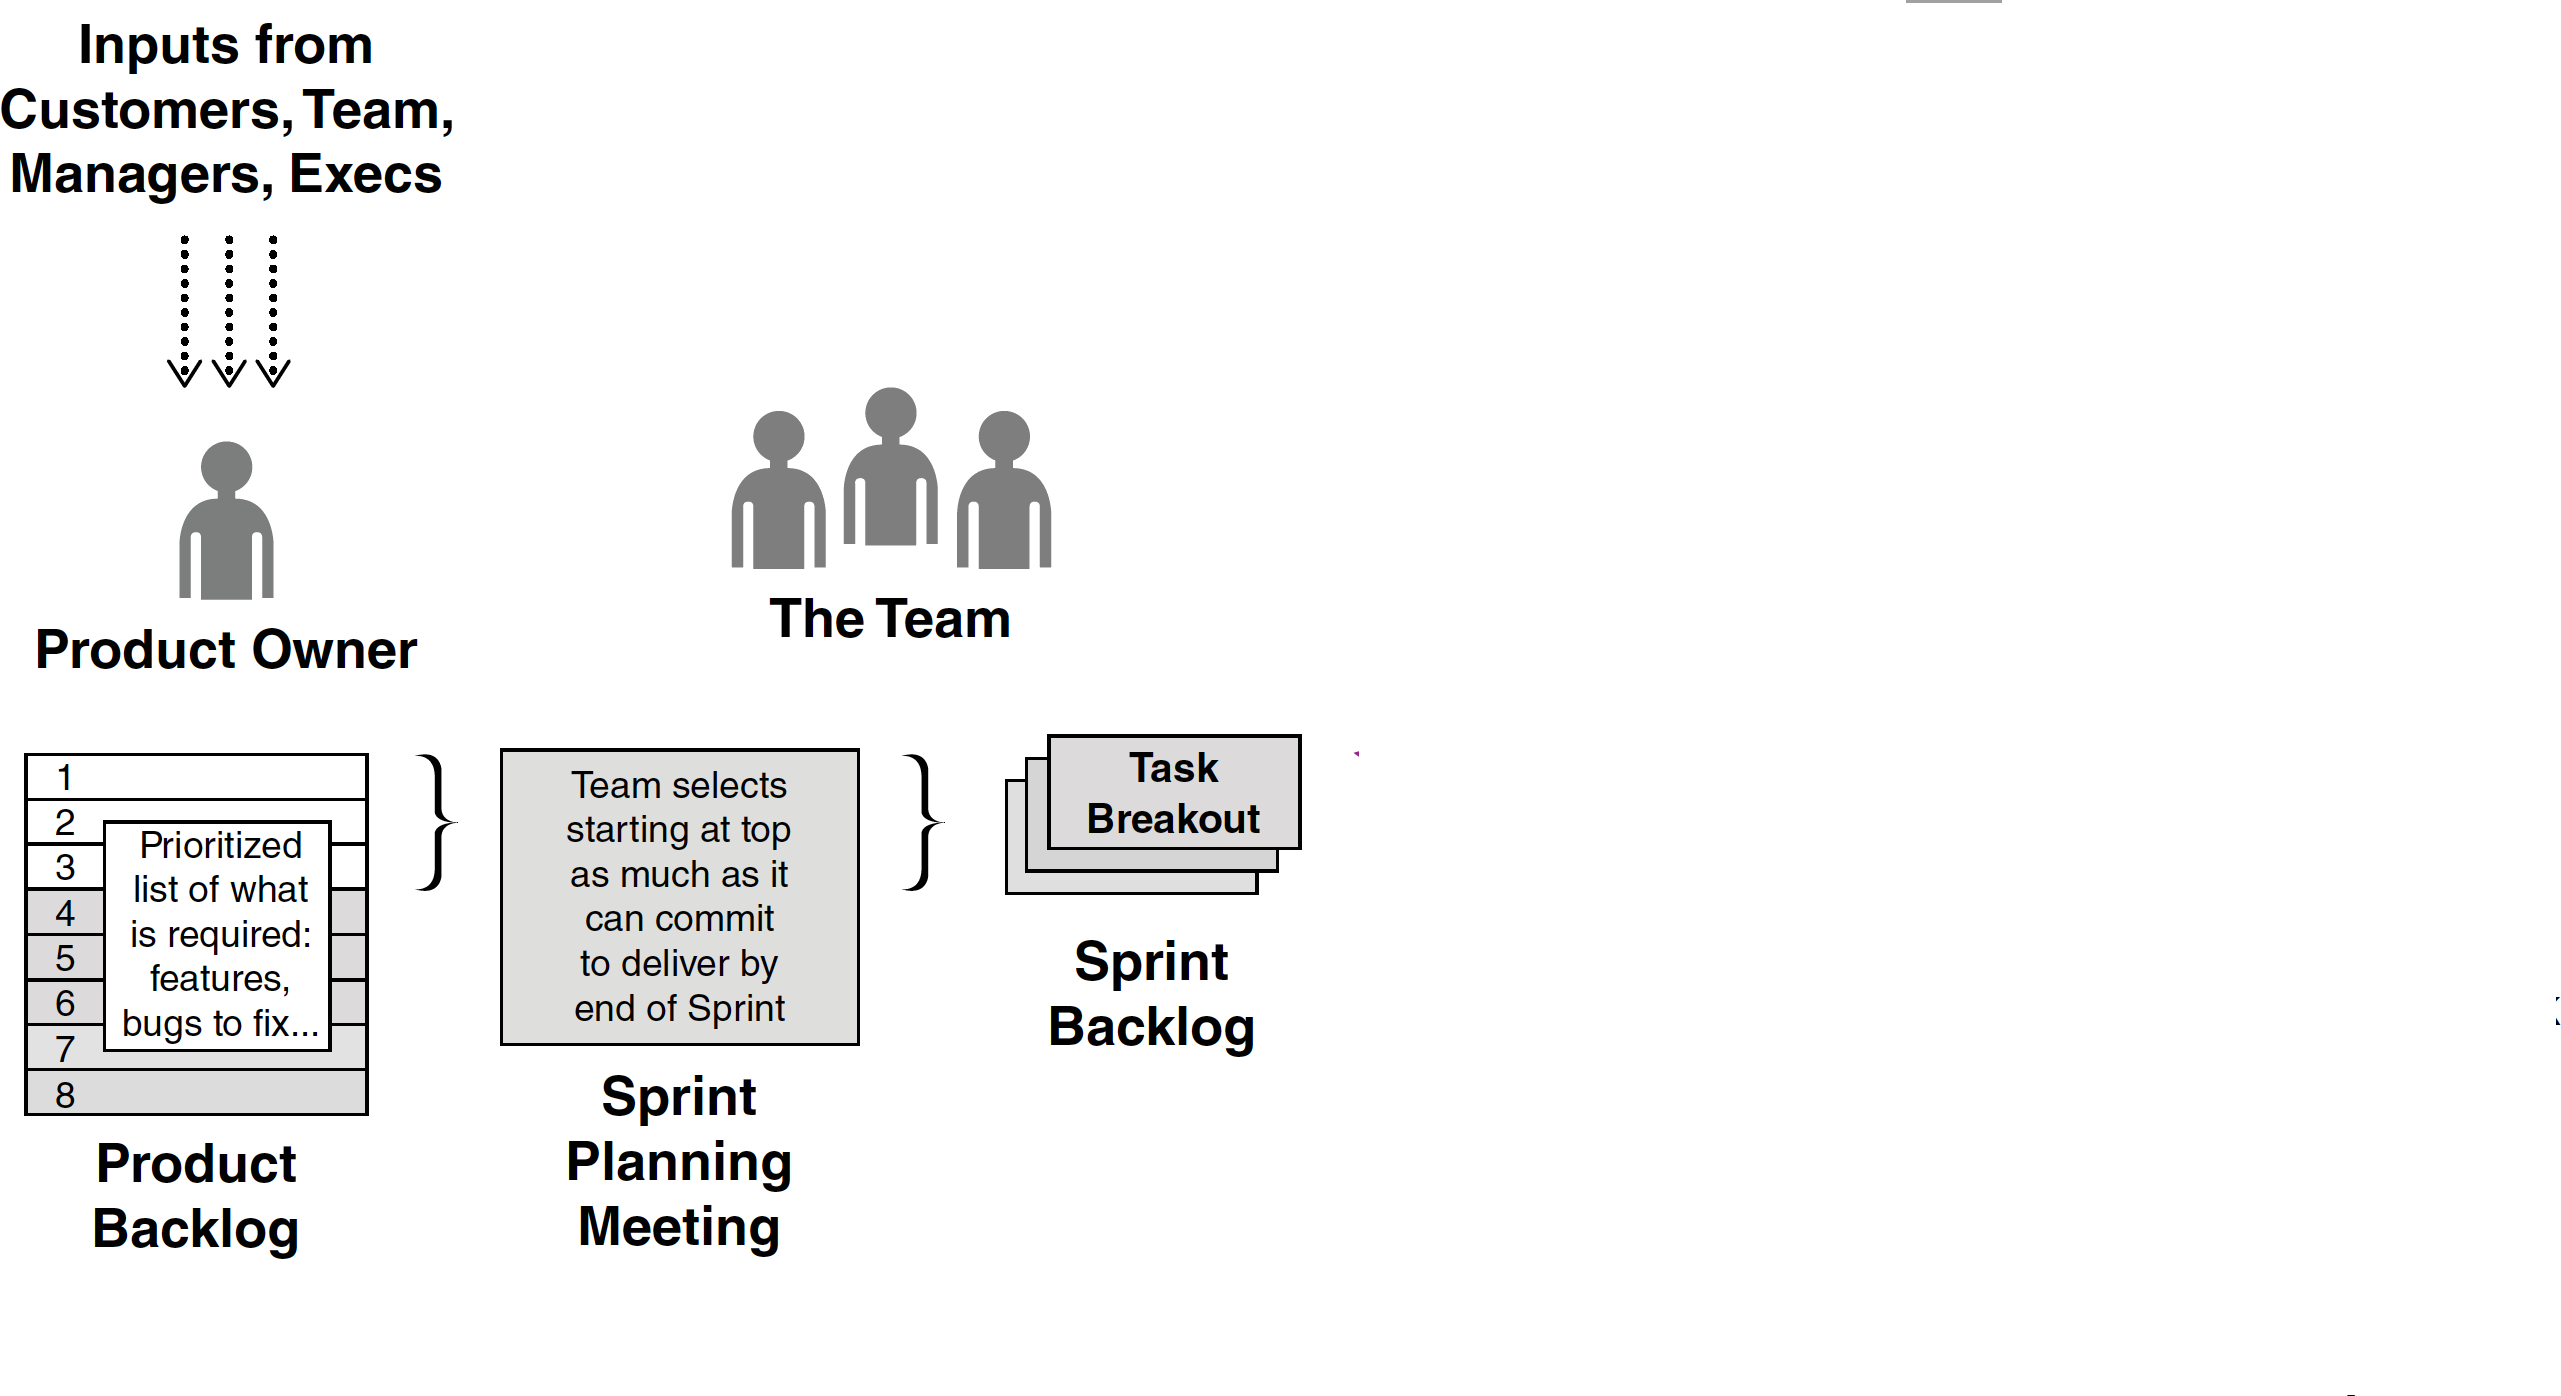
\includegraphics[scale=0.235]{../Figuras/flujo_scrum_2}
	\end{figure}
	\decoRule \\
  	\tiny \textit{Charles G Cobb. The project manager’s guide to mastering Agile: Principles and practices for an adaptive approach. John Wiley \& Sons, 2015.} \\
\end{frame}

\begin{frame}{Flujo del desarrollo}
	\begin{figure}
		\centering
	    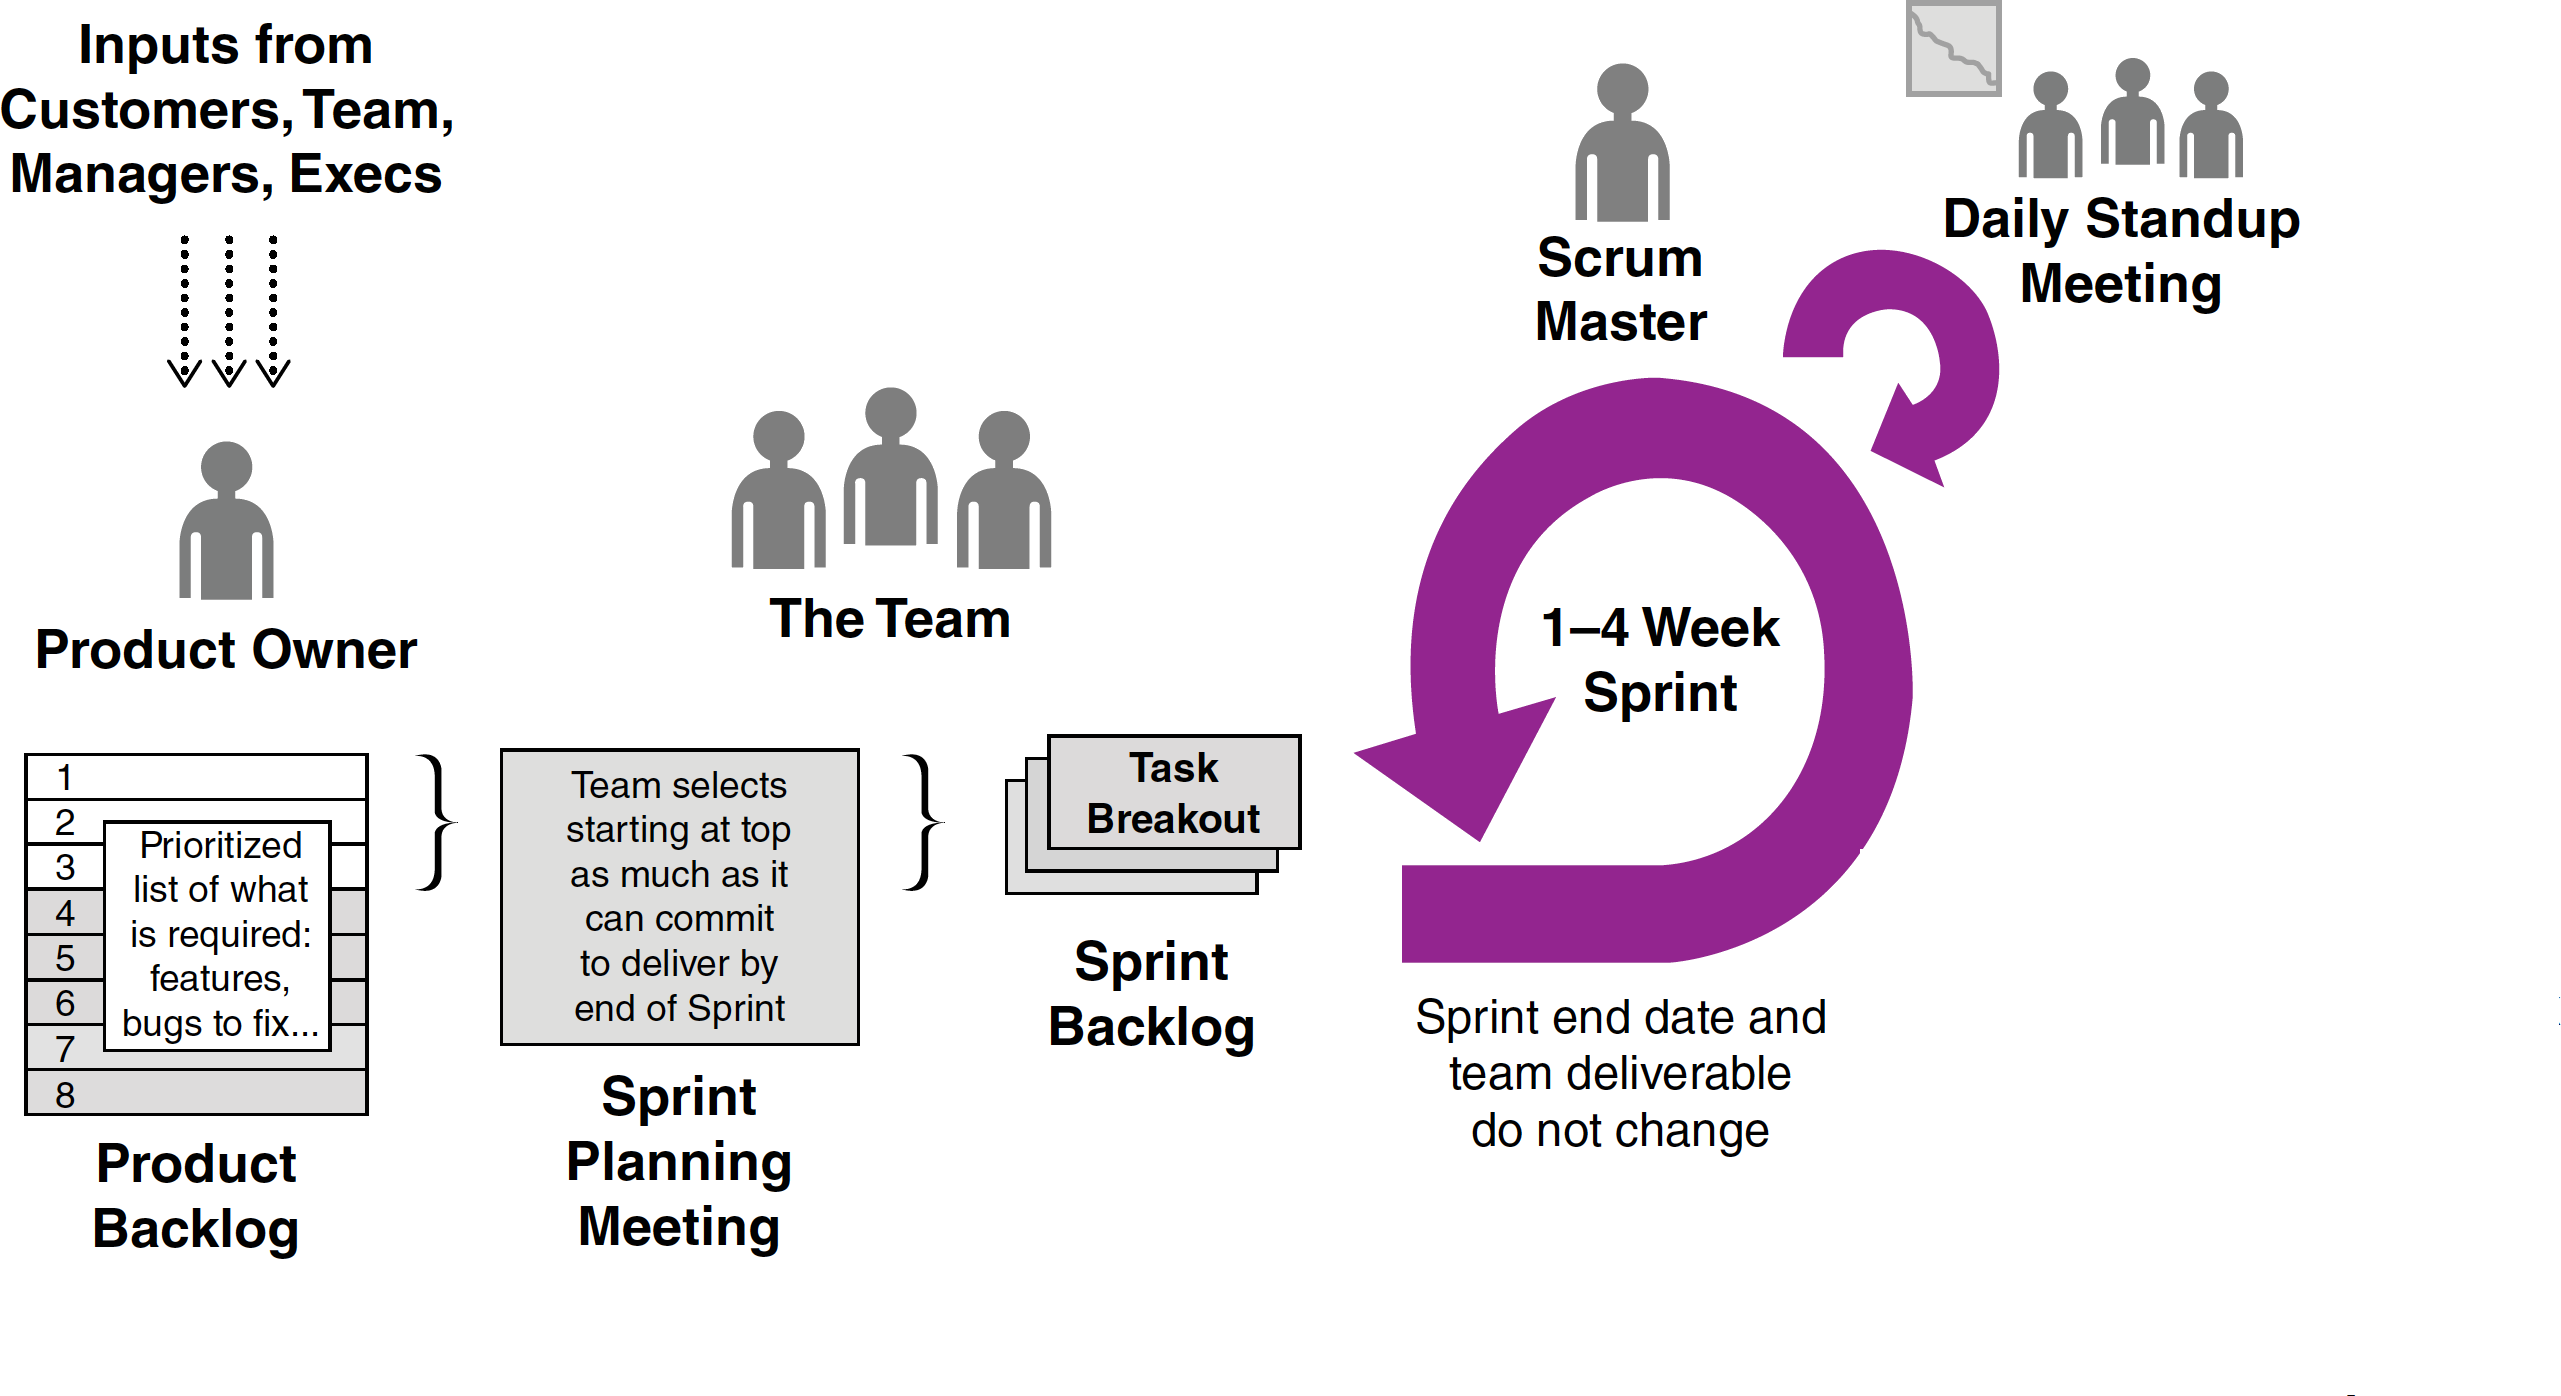
\includegraphics[scale=0.235]{../Figuras/flujo_scrum_3}
	\end{figure}
	\decoRule \\
  	\tiny \textit{Charles G Cobb. The project manager’s guide to mastering Agile: Principles and practices for an adaptive approach. John Wiley \& Sons, 2015.} \\
\end{frame}

\begin{frame}{Flujo del desarrollo}
	\begin{figure}
		\centering
	    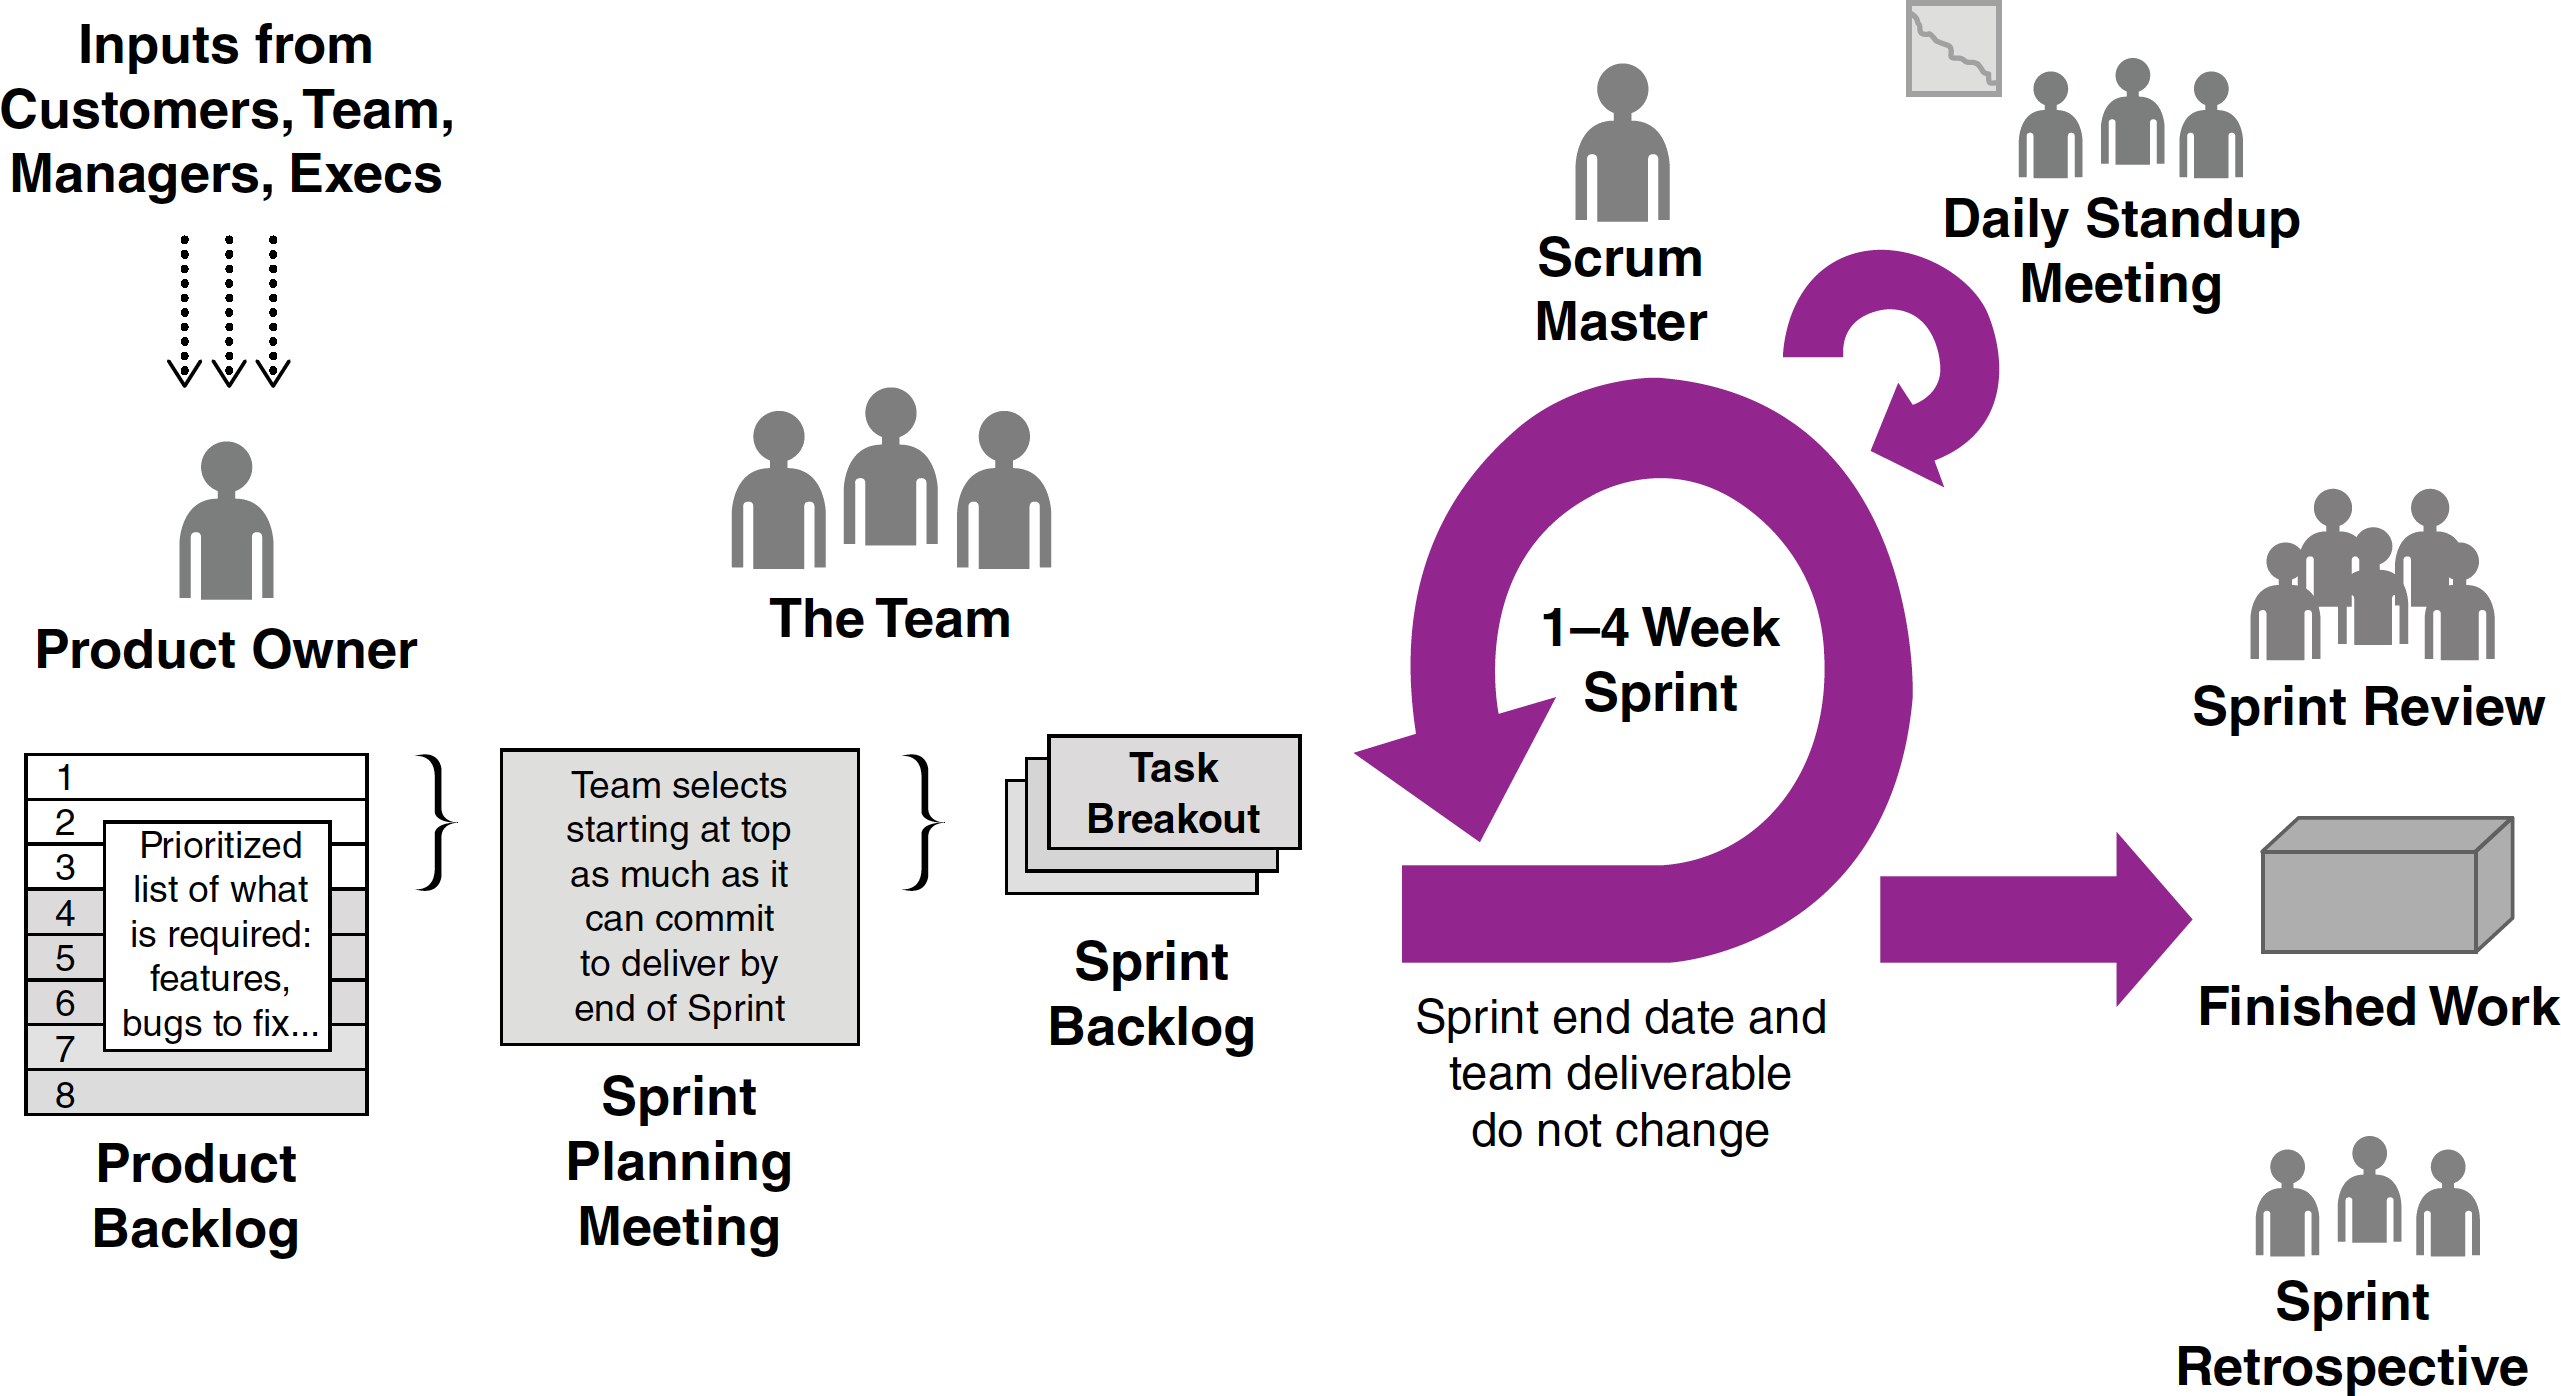
\includegraphics[scale=0.235]{../Figuras/flujo_scrum_4}
	\end{figure}
	\decoRule \\
  	\tiny \textit{Charles G Cobb. The project manager’s guide to mastering Agile: Principles and practices for an adaptive approach. John Wiley \& Sons, 2015.} \\
\end{frame}

\begin{frame}{Aportes}
	\begin{figure}
		\centering
		\begin{tikzpicture}[scale=0.8]
			\pie [rotate = 180] {45/Historias de usuario, 48.3/Fallas, 6.7/Mejoras}
		\end{tikzpicture}
	\end{figure}
\end{frame}

\begin{frame}{Aportes}
	\begin{figure}
		\centering
		\begin{tikzpicture}[scale=0.8]
			\pie [rotate = 180] {85.2/Terminada, 14.8/Reabierta}
		\end{tikzpicture}
	\end{figure}
\end{frame}

% VALIDACIÓN DEL DESARROLLO
\section{Validación del desarrollo}
\subsection{Revisión de las historias de usuario}
\begin{frame}
	\begin{itemize}[<+- | alert@+>]
	    \item Revisión por pares
	    \item Pruebas automatizadas
	    \item Revisión por parte del equipo de validación
	\end{itemize}
\end{frame}

\subsection{Revisión por parte del equipo de validación}
\begin{frame}{Revisión por parte del equipo de validación}
	\begin{figure}
		\centering
	    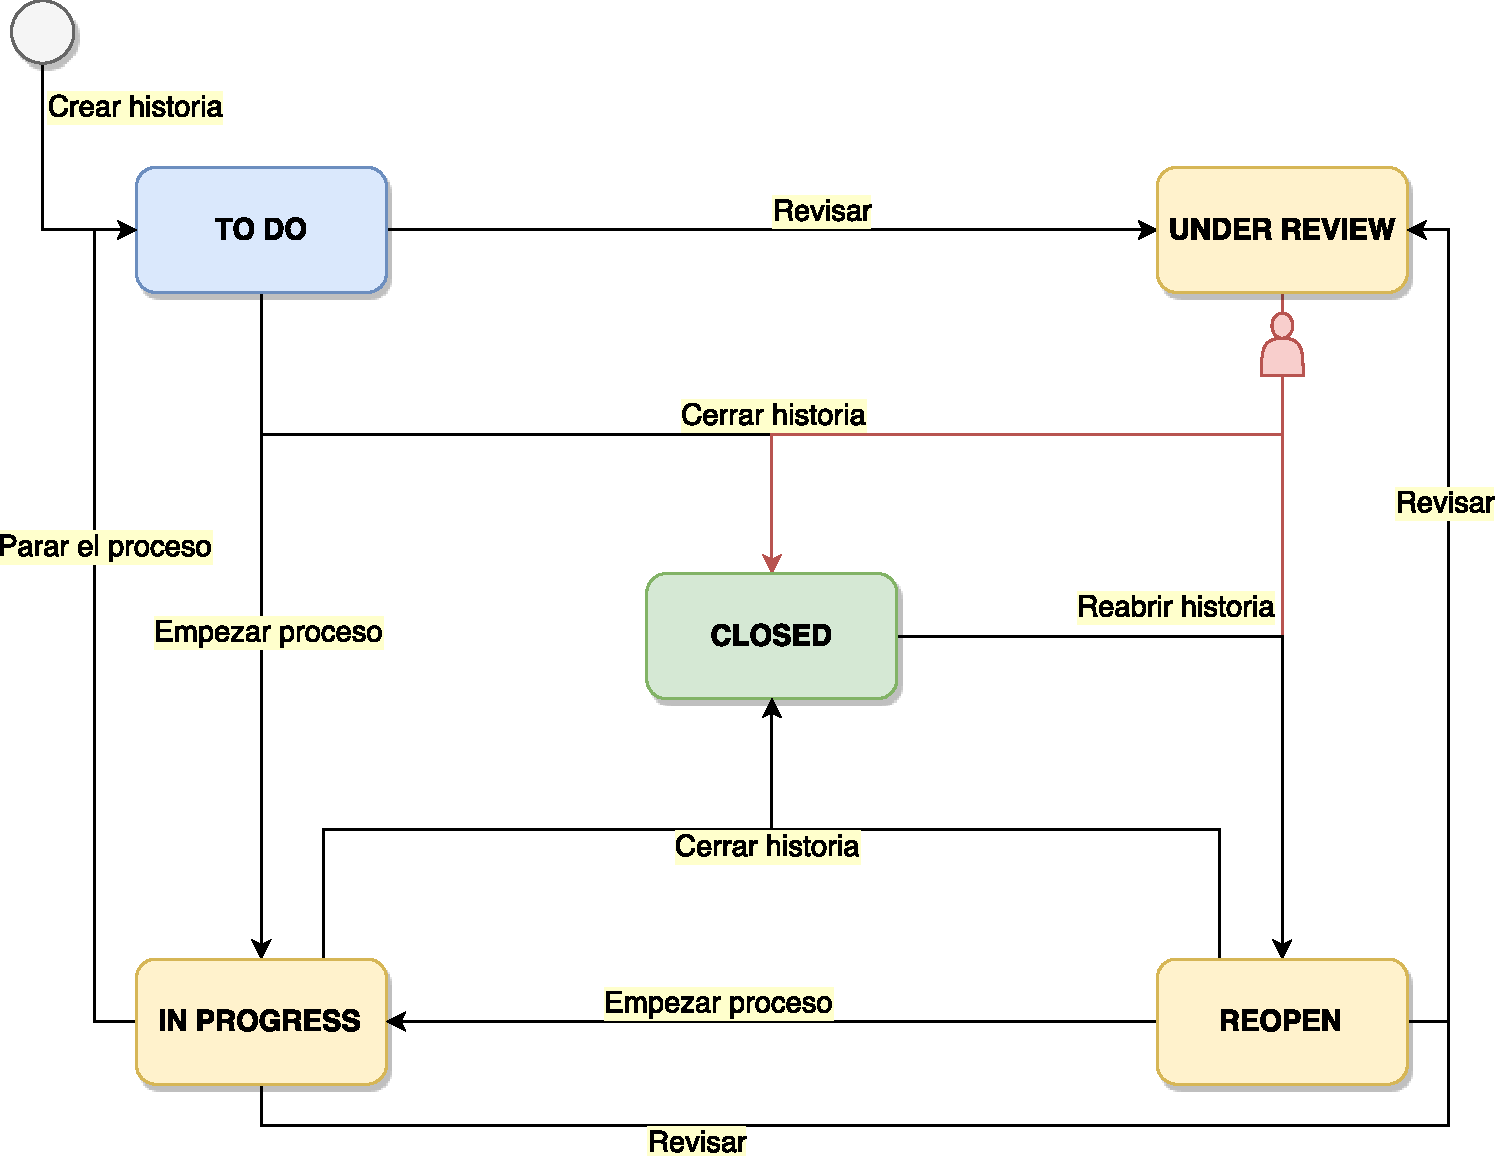
\includegraphics[scale=0.35]{../Figuras/workflow}
	\end{figure}
\end{frame}


% CONCLUSIÓN Y APORTES
\section{Conclusión y aportes}
\subsection{Conclusión}
\begin{frame}{Aportes}
	\begin{itemize}[<+- | alert@+>]
	    \item Reduce el tiempo de diseño y validación de material curricular.
	    \item Facilita la comunicación entre encargados del diseño y validación de los formularios.
	\end{itemize}
\end{frame}

\subsection{Trabajos futuros}
\begin{frame}{Trabajos futuros}
	\begin{itemize}[<+- | alert@+>]
	    \item Importador de cursos
	    \item Migración de motor de base de datos de los flujos de trabajo
	    \item Accesso de información a través de API pública
	    \item Catálogo de cursos
	    \item Flujo de trabajo para evaluaciones
	\end{itemize}
\end{frame}


\begin{frame}[standout]
  ¡Gracias por su atención!
\end{frame}


\end{document}
